% ===========================================================================
% Authorship Attribution and Style Fingerprinting in Bangla Literature
% KUET, Department of CSE -- CSE 4122 Natural Language Processing Laboratory
%
% Compile with XeLaTeX (required: fontspec + the vendored Bengali font):
%     latexmk -xelatex report.tex
%
% reports/numbers.tex is generated by scripts/make_report.py from the run's
% artifacts, so no figure in the prose is typed by hand.
% ===========================================================================
\documentclass[11pt]{article}
% ---------------------------------------------------------------------------
% Shared preamble.  Matches the visual language of the original proposal:
% one muted accent colour, a light panel fill, and nothing else.
% Compile with XeLaTeX -- fontspec and the Bengali font require it.
% ---------------------------------------------------------------------------
\usepackage[margin=0.95in]{geometry}
\usepackage{fontspec}
\usepackage{unicode-math}

\setmainfont{Latin Modern Roman}
\setmonofont{Latin Modern Mono}[Scale=0.9]

% Bengali is set in Noto Serif Bengali, vendored under reports/fonts so the
% document builds on a machine without it installed.
\newfontfamily\bengalifont{NotoSerifBengali-Regular.ttf}[Path=fonts/]
\newcommand{\bn}[1]{{\bengalifont #1}}

\usepackage{titlesec}
\usepackage{enumitem}
\usepackage{booktabs}
\usepackage{longtable}
\usepackage{graphicx}
\usepackage{float}
\usepackage{tikz}
\usetikzlibrary{arrows.meta, positioning, fit, calc}
\usepackage[most]{tcolorbox}
\usepackage{xcolor}
\usepackage{caption}
\usepackage{subcaption}
\usepackage{amsmath}
\usepackage{parskip}
\usepackage{microtype}
\usepackage[hidelinks]{hyperref}

\definecolor{accent}{HTML}{2F5D62}
\definecolor{panel}{HTML}{F4F4F4}
\definecolor{warn}{HTML}{B04A3F}
\definecolor{gold}{HTML}{9A7B1F}

\hypersetup{colorlinks=true, linkcolor=accent, urlcolor=accent, citecolor=accent}

\titleformat{\section}{\large\bfseries\color{accent}}{\thesection.}{0.5em}{}
\titlespacing*{\section}{0pt}{1.1em}{0.45em}
\titleformat{\subsection}{\bfseries}{\thesubsection}{0.5em}{}
\titlespacing*{\subsection}{0pt}{0.7em}{0.25em}
\titleformat{\subsubsection}[runin]{\bfseries\itshape}{}{0pt}{}[.]
\setlist{itemsep=1.5pt, topsep=3pt, parsep=0pt}

\captionsetup{font=small, labelfont={bf,color=accent}, skip=4pt}

% A boxed aside for the things a reader should not skim past.
\newtcolorbox{keybox}[1][]{
  colback=panel, colframe=accent, boxrule=0.6pt, arc=1.2mm,
  left=7pt, right=7pt, top=5pt, bottom=5pt,
  fonttitle=\bfseries\small, coltitle=white, #1}

\newtcolorbox{plainbox}{
  colback=panel, colframe=black!45, boxrule=0.4pt, arc=1mm,
  left=6pt, right=6pt, top=5pt, bottom=5pt}

% Generated by scripts/make_report.py -- do not edit by hand.

\newcommand{\CharOrder}{5}
\newcommand{\FTEpochs}{2}
\newcommand{\FTMaxLen}{192}
\newcommand{\PassageTokens}{220}
\newcommand{\PretrainedModel}{csebuetnlp/banglabert}
\newcommand{\Seed}{20242025}
\newcommand{\WordOrder}{3}
\newcommand{\WtvDim}{200}
\newcommand{\WtvNegative}{8}
\newcommand{\WtvWindow}{5}
\newcommand{\accLongDisc}{0.685}
\newcommand{\accLongGen}{0.792}
\newcommand{\accShortDisc}{0.551}
\newcommand{\accShortGen}{0.744}
\newcommand{\bertFTAcc}{0.775}
\newcommand{\bertFTAccPct}{77.5\%}
\newcommand{\bertFTFone}{0.763}
\newcommand{\bestAcc}{0.834}
\newcommand{\bestAccPct}{83.4\%}
\newcommand{\bestCI}{[0.806, 0.861]}
\newcommand{\bestFone}{0.843}
\newcommand{\bestModel}{Generative char-5-gram LM}
\newcommand{\booksTouched}{57}
\newcommand{\bothCorrect}{510}
\newcommand{\bothWrong}{27}
\newcommand{\chanceAcc}{0.200}
\newcommand{\chancePct}{20.0\%}
\newcommand{\comboBertAcc}{0.801}
\newcommand{\comboBertAccPct}{80.1\%}
\newcommand{\comboBertFone}{0.784}
\newcommand{\comboScratchAcc}{0.791}
\newcommand{\comboScratchAccPct}{79.1\%}
\newcommand{\comboScratchFone}{0.784}
\newcommand{\discOnlyCorrect}{56}
\newcommand{\earliestAuthor}{Ishwar Chandra Vidyasagar}
\newcommand{\genCharAcc}{0.834}
\newcommand{\genCharAccPct}{83.4\%}
\newcommand{\genCharFone}{0.843}
\newcommand{\genOnlyCorrect}{84}
\newcommand{\genWordAcc}{0.768}
\newcommand{\genWordAccPct}{76.8\%}
\newcommand{\genWordFone}{0.767}
\newcommand{\leakGap}{20.7\%}
\newcommand{\leakGapAbs}{0.207}
\newcommand{\lenLong}{220}
\newcommand{\lenShort}{40}
\newcommand{\meanPassageTokens}{231}
\newcommand{\mostChalit}{Abanindranath Tagore}
\newcommand{\mostSadhu}{Ishwar Chandra Vidyasagar}
\newcommand{\nAuthors}{5}
\newcommand{\nPassages}{2,955}
\newcommand{\nTest}{712}
\newcommand{\nTokens}{682,607}
\newcommand{\nTrain}{1,821}
\newcommand{\nVal}{422}
\newcommand{\nWorks}{42}
\newcommand{\paradigmAgreement}{75.4\%}
\newcommand{\passagesPerAuthor}{591}
\newcommand{\permCharDrop}{0.570}
\newcommand{\permFuncDrop}{0.008}
\newcommand{\permPosDrop}{0.027}
\newcommand{\permStructDrop}{0.008}
\newcommand{\permTopFamily}{character $n$-grams}
\newcommand{\posAcc}{87.2\%}
\newcommand{\posAccRaw}{0.872}
\newcommand{\posRecallAdp}{50\%}
\newcommand{\posRecallNoun}{82\%}
\newcommand{\posRecallPart}{78\%}
\newcommand{\posRecallPron}{98\%}
\newcommand{\posRecallPunct}{100\%}
\newcommand{\posRecallVerb}{97\%}
\newcommand{\posSentences}{56}
\newcommand{\posTokens}{320}
\newcommand{\proofreadRate}{95.7\%}
\newcommand{\randomSplitAcc}{0.993}
\newcommand{\scanPagesProofread}{7,158}
\newcommand{\scanPagesSeen}{7,480}
\newcommand{\silBertAuthor}{0.143}
\newcommand{\silBertRatio}{0.71}
\newcommand{\silBertWork}{0.201}
\newcommand{\silScratchMeanAuthor}{0.255}
\newcommand{\silScratchMeanRatio}{0.80}
\newcommand{\silScratchMeanWork}{0.320}
\newcommand{\silScratchSifAuthor}{0.264}
\newcommand{\silScratchSifRatio}{0.82}
\newcommand{\silScratchSifWork}{0.320}
\newcommand{\svmAllAcc}{0.795}
\newcommand{\svmAllAccPct}{79.5\%}
\newcommand{\svmAllFone}{0.790}
\newcommand{\svmBertAcc}{0.772}
\newcommand{\svmBertAccPct}{77.2\%}
\newcommand{\svmBertFone}{0.751}
\newcommand{\svmCharAcc}{0.778}
\newcommand{\svmCharAccPct}{77.8\%}
\newcommand{\svmCharFone}{0.773}
\newcommand{\svmFuncAcc}{0.726}
\newcommand{\svmFuncAccPct}{72.6\%}
\newcommand{\svmFuncFone}{0.720}
\newcommand{\svmPosAcc}{0.611}
\newcommand{\svmPosAccPct}{61.1\%}
\newcommand{\svmPosFone}{0.602}
\newcommand{\svmScratchMeanAcc}{0.756}
\newcommand{\svmScratchMeanAccPct}{75.6\%}
\newcommand{\svmScratchMeanFone}{0.742}
\newcommand{\svmScratchSifAcc}{0.767}
\newcommand{\svmScratchSifAccPct}{76.7\%}
\newcommand{\svmScratchSifFone}{0.756}
\newcommand{\svmStructAcc}{0.801}
\newcommand{\svmStructAccPct}{80.1\%}
\newcommand{\svmStructFone}{0.799}
\newcommand{\testFrac}{24.1\%}
\newcommand{\trainFrac}{61.6\%}
\newcommand{\valFrac}{14.3\%}
\newcommand{\workSplitAcc}{0.787}


\begin{document}

% ---------------------------------------------------------------- title page
\begin{titlepage}
\centering
\vspace*{1.2cm}

{\large Khulna University of Engineering \& Technology}\\[2pt]
{\normalsize Department of Computer Science and Engineering}\\[1.6cm]

\rule{\linewidth}{0.6pt}\\[10pt]
{\LARGE\bfseries Authorship Attribution and\\[3pt] Style Fingerprinting in
Bangla Literature}\\[10pt]
{\large\color{accent} Project Report}\\[6pt]
\rule{\linewidth}{0.6pt}\\[1.4cm]

{\normalsize Course No: CSE 4122 \quad$\cdot$\quad Course Title: Natural
Language Processing Laboratory}\\[1.8cm]

\begin{minipage}[t]{0.47\linewidth}
\raggedright
\textbf{Submitted To}\\[6pt]
Dr.\ K.\ M.\ Azharul Hasan\\
{\small Professor, Department of Computer Science and Engineering,\\
KUET, Khulna}\\[10pt]
Md.\ Nazirulhasan Shawon\\
{\small Assistant Professor, Department of Computer Science and Engineering,\\
KUET, Khulna}
\end{minipage}\hfill
\begin{minipage}[t]{0.47\linewidth}
\raggedright
\textbf{Submitted By}\\[6pt]
Abu Daud Sharif\\
{\small Roll: 2107002}\\[8pt]
Sheikh Md.\ Galib Mahim\\
{\small Roll: 2107020}\\[10pt]
{\small Section: A \quad Lab Group: A1\\
Year: 4th \quad Term: 1st\\
Session: 2024-25}
\end{minipage}

\vfill

\end{titlepage}

\tableofcontents
\newpage

% ===========================================================================
% Method sections.  Every number is a macro from numbers.tex; nothing typed.
% ===========================================================================

\section{Introduction}

Authorship attribution asks a simple question: given a piece of text and a list of possible authors, who wrote it? But just guessing the name isn't enough. A good system should also explain \emph{why} it made that choice. If it can point out specific sentence lengths, common words, or character patterns, it is doing real stylometry. If it just gives a label without reasons, it acts like a black box.

Bangla makes this task harder than English. It is a morphologically rich language, meaning words change forms a lot. A model that only looks at whole words might get confused by different forms of the same word. Bangla also uses the \emph{dari} (\bn{।}) instead of a full stop, has its own numbers, and has two main writing styles: \bn{সাধু} (literary) and \bn{চলিত} (colloquial). This difference in writing styles is actually a huge clue for figuring out who the author is.

This project builds a system to identify \nAuthors{} Bangla authors. We compare two main ways to solve this:

\begin{itemize}
  \item a \textbf{generative} approach: we build a language model for each author and check which model finds the text least surprising;
  \item a \textbf{discriminative} approach: we train models to draw a line between authors. We test several models, from simple Naive Bayes and SVMs to deep learning models like a BiLSTM and a fine-tuned BanglaBERT.
\end{itemize}

\paragraph{Scope of the task.}
We set clear rules for our experiment:
\begin{itemize}
  \item \textbf{Closed-set formulation:} We only try to pick between our \nAuthors{} chosen authors based on their literary work. If a fourth author wrote the text, our system will still pick one of the three.
  \item \textbf{Focus on style:} The goal is to learn the author's writing style, not to check for copied text or plagiarism.
  \item \textbf{Known limits:} Section \ref{sec:limitations} honestly discusses the flaws and limits of our approach.
\end{itemize}

\subsection{Why we chose these three authors}

We picked three very famous writers: Rabindranath Tagore (1861--1941), Kazi Nazrul Islam (1899--1976) and Humayun Ahmed (1948--2012). We did this for two main reasons.

First, \emph{people know them}. Even if you don't run our code, you probably know how these authors write. This makes it easier for you to judge if our system's answers make sense.

Second, \emph{they write differently}. These authors span over a century and use different writing styles. This helps our models learn, but as we explain in Section \ref{sec:limitations}, it also means our models are partly just guessing the time period, rather than just the personal style.

\section{How we built the dataset}

\subsection{Getting the books and splitting the data}

We downloaded \nBooks{} books (three per author) from a public Bengali e-library. Since the website's links are unpredictable, we built a scraper to find all the chapter pages from the main book index. We saved everything we downloaded, so it is cheap and easy to run the code again.

The most important decision was made \emph{before we downloaded anything}. For each author, we picked two books for \textbf{training} the models and one book to be \textbf{held out} (kept completely unseen):

\begin{center}\small
\begin{tabular}{lll}
\toprule
\textbf{Author} & \textbf{Training books} & \textbf{Held out} \\
\midrule
Rabindranath Tagore & \bn{গল্পগুচ্ছ}, \bn{সাধনা} & \bn{রহস্য সমগ্র} \\
Kazi Nazrul Islam & \bn{কুহেলিকা}, \bn{রিক্তের বেদন} & \bn{ব্যথার দান} \\
Humayun Ahmed & \bn{হিমু}, \bn{বিপদ} & \bn{হিমুর হাতে কয়েকটি নীলপদ্ম} \\
\bottomrule
\end{tabular}
\end{center}

These \nUnseenBooks{} held-out books \emph{are} our test set. Our models never see them during training. We didn't use them to build our vocabulary, our word embeddings, or anything else. You can verify this yourself by looking at the \texttt{corpus/unseen/} folder.

We also saved the entire dataset as plain UTF-8 text files, so you can easily read or copy text from them.

\subsection{Cleaning the text}

Web pages have extra stuff like menus and captions. We only kept paragraphs that were at least 30 characters long, and where mostly all characters were actual Bangla letters. This step helped remove English text and transliterations. After that, we cleaned up the Bangla text: we fixed inconsistent characters, made quotation marks uniform, and replaced all numbers with a placeholder so the models wouldn't cheat by memorizing chapter numbers.

\subsection{The reprint problem}
\label{sec:overlap}

While making the dataset, we found a big problem that forced us to change our code.

Bengali publishers often reprint old stories in new collections. It turned out that Tagore's held-out book, \bn{\overlapUnseenBook{}}, was an anthology that included stories from his training book, \bn{\overlapTrainBook{}}. If we ignored this, our models would have been tested on stories they had already memorized during training. All our results for Tagore would have been fake.

We couldn't just check story titles, because the punctuation in the titles sometimes changed. Instead, we checked the actual text. We broke each chapter into chunks of 10 words (shingles) and checked how many chunks from the training chapters appeared in the held-out chapters.

\paragraph{Choosing the right chunk step (stride).}
We had to be careful about how we stepped through the text to make our chunks:
\begin{itemize}
  \item \textbf{Taking steps of 5 (failed):} At first, we grabbed a 10-word chunk every 5 words. But if one version of a story had just one extra word, all the following chunks wouldn't match. Matching stories scored very low.
  \item \textbf{Taking steps of 1 (worked):} When we moved forward by just 1 word at a time, we caught all the matching text. The same stories matched perfectly (scoring \overlapRange{}), while different stories scored exactly 0.
\end{itemize}

We found \nOverlapHits{} training chapters that were reprinted in the held-out books. We deleted them \textbf{from the training set}. We never touched the held-out books, because it is crucial that our test set remains completely unseen and pure.

\subsection{Cutting text into passages}

We test our models on \emph{passages} of about \PassageTokens{} words. We cut the text at the end of sentences, and we never cross over into a new chapter. We chose this size because the author with the least data only has about 30,000 training words, so making the pieces bigger would leave us with too little training data. Also, \PassageTokens{} words is about the size of a standard paragraph, which is what users will likely test in our app. We throw away any passage that is shorter than \MinPassageTokens{} words.

After cleaning, we had \nPassages{} passages from \nChapters{} chapters, giving us a total of \nTokens{} words. You can already see differences between the authors just by looking at sentence length: \longestSentAuthor{}'s sentences average \longestSentLen{} words, while \shortestSentAuthor{}'s average only \shortestSentLen{} words.

\begin{table}[H]
\centering\small
\caption{The dataset, book by book. It is unbalanced, with Tagore having much more text than Humayun Ahmed. This is why we use class weights during training instead of deleting text.}
\label{tab:corpus}
% Generated by scripts/05_report_artifacts.py -- do not edit by hand.
\begin{tabular}{lllrrr}
\toprule
\textbf{Author} & \textbf{Book} & \textbf{Role} & \textbf{Chapters} & \textbf{Tokens} & \textbf{Passages} \\
\midrule
Rabindranath Tagore & \bn{গল্পগুচ্ছ} & train & 44 & 101,637 & 766 \\
Rabindranath Tagore & \bn{সাধনা: জীবনের উপলব্ধি} & train & 9 & 35,885 & 269 \\
Kazi Nazrul Islam & \bn{কুহেলিকা} & train & 20 & 28,829 & 223 \\
Kazi Nazrul Islam & \bn{রিক্তের বেদন} & train & 8 & 22,044 & 171 \\
Humayun Ahmed & \bn{হিমু} & train & 13 & 17,216 & 138 \\
Humayun Ahmed & \bn{বিপদ} & train & 6 & 11,333 & 92 \\
\midrule
Rabindranath Tagore & \bn{রহস্য সমগ্র} & \textbf{held out} & 12 & 23,404 & 179 \\
Kazi Nazrul Islam & \bn{ব্যথার দান} & \textbf{held out} & 6 & 23,147 & 179 \\
Humayun Ahmed & \bn{হিমুর হাতে কয়েকটি নীলপদ্ম} & \textbf{held out} & 13 & 22,552 & 179 \\
\bottomrule
\end{tabular}

\end{table}

Table \ref{tab:corpus} shows our full dataset. The three rows labeled \emph{held out} make up our entire test set.

\section{Preparing text and extracting features}

\subsection{Breaking text into tokens}

We split sentences using the dari, double dari, question marks, and exclamation points. We only split on Latin full stops if a space and a letter follow them, because full stops are also used in abbreviations. When breaking sentences into words, we keep hyphenated Bangla words together and replace all numbers with a special token.

\subsection{Four types of features}

We grouped our features into four categories so we can easily test which ones matter most.

\paragraph{Function words (\texttt{fw:}).} We look at the frequencies of the \TopFunctionWords{} most common connecting words. While topic classifiers usually delete these words, they are great for identifying authors. An author can easily change what they are writing about, but it is hard for them to change which basic grammar words they unconsciously use.

\paragraph{Structural stats (\texttt{st:}).} We look at sentence lengths, word lengths, unique vocabulary size, punctuation use, and how often the author uses \bn{সাধু} (literary) versus \bn{চলিত} (colloquial) words.

\paragraph{Character patterns (\texttt{ch:}).} We count small sequences of 2 to 4 characters (character n-grams). Since Bangla changes word endings to show grammar, these small character chunks are very powerful. They help the model recognize grammatical tenses even if it hasn't seen the exact full word before.

\paragraph{Grammar tags (\texttt{pos:}).} We check patterns in Parts of Speech (like nouns, verbs, etc.). Since there wasn't a good ready-made Bangla tagger available for our setup, we built a simple rule-based one. It achieves \posAcc{} accuracy on the only available Bengali treebank dataset (which has \posTokens{} words in \posSentences{} sentences).

\section{The four models}
\label{sec:models}

We trained a dozen models, but we focus on \textbf{four} of them in this report. We picked these four because they show a clear progression: each model is capable of doing something the previous one could not. This makes it easy to understand why the accuracy changes.

\begin{center}\small
\begin{tabular}{llp{6.1cm}}
\toprule
\textbf{Model} & \textbf{Lab} & \textbf{What it looks at} \\
\midrule
Naive Bayes (word counts)      & 2, 3 & Which words appear, and how often \\
TF--IDF unigrams + SVM   & 2, 3 & Same as above, but gives more weight to rare, useful words \\
BiLSTM                      & 4    & The \emph{order} of the words \\
BanglaBERT, fine-tuned      & 5    & Everything above, plus it already knows Bangla from huge outside datasets \\
\bottomrule
\end{tabular}
\end{center}

We talk about our other models (like the Kneser-Ney language models and from-scratch Transformers) in Section \ref{sec:alsoran}.

\subsection{Naive Bayes using word counts}

We wrote this model from scratch using NumPy instead of relying on a library. It calculates the probability of each author given the words in a passage. We do the math in log space to prevent the tiny probabilities from breaking the computer's math limits.

\paragraph{Why we used whole words for Naive Bayes.}
Even though character chunks work great for Bangla, we used whole words for Naive Bayes for practical reasons:
\begin{itemize}
  \item \textbf{Easy to read:} You can look at the word scores and clearly see which specific vocabulary words made the model pick a certain author.
  \item \textbf{It works well:} On our dataset, word-level Naive Bayes scored \naiveBayesAcc{}, beating the character version which scored \naiveBayesCharAcc{}.
\end{itemize}

We also used add-$\alpha$ smoothing. Without it, if the model saw one word that an author had never used in training, it would instantly give that author a 0\% chance, even if the rest of the text strongly matched their style.

\subsection{TF--IDF unigrams with a linear SVM}

This model uses the same word counts, but it weights them. If a word is very common for one author but rare everywhere else, it gets a higher score. It then draws a strict mathematical line (a maximum-margin boundary) to separate the authors.

This model is our baseline for checking how much the topic matters. Since it only looks at individual words, its accuracy tells us how much of the problem can be solved just by looking at vocabulary alone.

\subsection{BiLSTM}

This is the first model that actually pays attention to the \emph{order} of words. It reads the text forwards and backwards. Instead of just looking at the final state of the reading process, it takes an average across the whole passage. This is important because an author's style is spread throughout the text, not just at the very end.

We trained its word embeddings from scratch using only our training data. It started with random knowledge and only learned from our six books. This makes it a fair comparison for the next model.

\subsection{BanglaBERT, fine-tuned}

\begin{figure}[H]
\centering
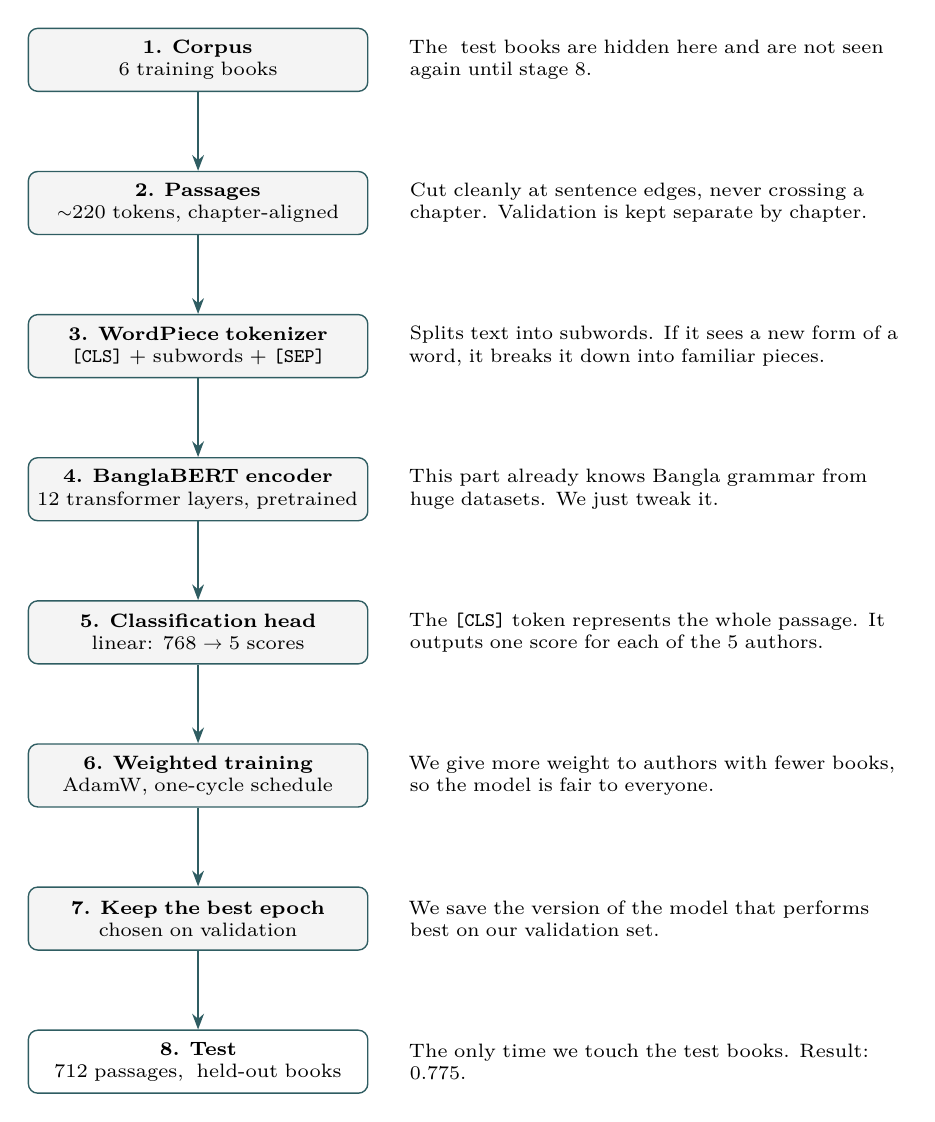
\begin{tikzpicture}[
  font=\scriptsize,
  stage/.style={draw=accent, fill=panel, rounded corners=1.2mm, line width=0.5pt,
                text width=4.1cm, align=center, minimum height=8mm, inner sep=3pt},
  note/.style={text width=6.2cm, align=left, font=\scriptsize},
  arr/.style={-{Stealth[length=2mm]}, draw=accent, line width=0.6pt},
]
\node[stage] (s1) {\textbf{1. Corpus}\\6 training books};
\node[stage, below=10mm of s1] (s2) {\textbf{2. Passages}\\$\sim$\PassageTokens{} tokens, chapter-aligned};
\node[stage, below=10mm of s2] (s3) {\textbf{3. WordPiece tokenizer}\\\texttt{[CLS]} + subwords + \texttt{[SEP]}};
\node[stage, below=10mm of s3] (s4) {\textbf{4. BanglaBERT encoder}\\12 transformer layers, pretrained};
\node[stage, below=10mm of s4] (s5) {\textbf{5. Classification head}\\linear: 768 $\rightarrow$ \nAuthors{} scores};
\node[stage, below=10mm of s5] (s6) {\textbf{6. Weighted training}\\AdamW, one-cycle schedule};
\node[stage, below=10mm of s6] (s7) {\textbf{7. Keep the best epoch}\\chosen on validation};
\node[stage, below=10mm of s7, fill=white] (s8) {\textbf{8. Test}\\\nTest{} passages, \nUnseenBooks{} held-out books};

\foreach \a/\b in {s1/s2, s2/s3, s3/s4, s4/s5, s5/s6, s6/s7, s7/s8}
  \draw[arr] (\a) -- (\b);

\node[note, right=4mm of s1] {The \nUnseenBooks{} test books are hidden here and are not seen again until stage 8.};
\node[note, right=4mm of s2] {Cut cleanly at sentence edges, never crossing a chapter. Validation is kept separate by chapter.};
\node[note, right=4mm of s3] {Splits text into subwords. If it sees a new form of a word, it breaks it down into familiar pieces.};
\node[note, right=4mm of s4] {This part already knows Bangla grammar from huge datasets. We just tweak it.};
\node[note, right=4mm of s5] {The \texttt{[CLS]} token represents the whole passage. It outputs one score for each of the \nAuthors{} authors.};
\node[note, right=4mm of s6] {We give more weight to authors with fewer books, so the model is fair to everyone.};
\node[note, right=4mm of s7] {We save the version of the model that performs best on our validation set.};
\node[note, right=4mm of s8] {The only time we touch the test books. Result: \bertFTAcc{}.};
\end{tikzpicture}
\caption{How we fine-tuned BanglaBERT. It shares the first two steps with other models, but uses a powerful pre-trained engine to process the text.}
\label{fig:bertarch}
\end{figure}

This model (\PretrainedModel{}) was pre-trained on a massive amount of Bangla text before it ever saw our project. We just added a final layer to make it output a probability for each of our authors.

Two important details in Figure \ref{fig:bertarch}: First, in stage 3, it breaks text into \emph{subwords}. This means if it sees a word with a new ending, it doesn't get totally confused; it just breaks the word down into familiar pieces. Second, in stage 6, we give more weight to the authors who have less data in our training set, so the model doesn't just blindly guess the author who wrote the most books.

\section{How we ran the experiment}

\subsection{Splitting the data fairly}

Our test set consists of the \nUnseenBooks{} held-out books. We balanced it to have exactly \testPerAuthor{} passages per author. Because it's perfectly balanced, random guessing would score exactly \chanceAcc{}.

For validation (to decide when to stop training), we used parts of the \emph{training} books. We made sure to hold out \textbf{whole chapters} for validation. If we just mixed all passages together and grabbed some randomly for validation, the model might see the first half of a chapter during training and the second half during validation, which is cheating.

The training set is \emph{not} balanced. If we threw away Tagore's data just to match our smallest author, we'd lose too much valuable information. Instead, we show the models everything and just adjust their internal weights. In the end, we had \nTrain{} training passages, \nVal{} validation passages, and \nTest{} test passages.

\subsection{Where the code ran}

The simpler models trained on our local CPU in about two minutes. The heavy deep learning models (BanglaBERT, BiLSTM, and Transformer) ran remotely on Kaggle using a GPU. We made sure the Kaggle job used the exact same train/test splits as our local computer, so they were working on the exact same problem. When we collected the Kaggle results, our local script double-checked the accuracy to make sure no mistakes were made.

\subsection{Reproducibility}

Every random choice in the code is locked to a specific seed (\texttt{SEED = \Seed{}}). If you run our code again on your machine, you will get the exact same numbers shown in this report.

% ===========================================================================
% Results sections.  Every number is a macro from numbers.tex; nothing typed.
% ===========================================================================

\section{Results}
\label{sec:results}

All the results below are based on our test set: \nTest{} passages taken from the \nUnseenBooks{} completely unseen books. We have \testPerAuthor{} passages per author, meaning a random guess would get \chanceAcc{} right. No model saw a single word from these books during training.

\subsection{The four main models}

\begin{table}[H]
\centering\small
\caption{Our four main models, ordered by how much information they use. Random guessing scores \chanceAcc{}.}
\label{tab:main}
\begin{tabular}{llrr}
\toprule
\textbf{Model} & \textbf{What it adds} & \textbf{Accuracy} & \textbf{Macro F1} \\
\midrule
Naive Bayes (word counts)   & word counts            & \naiveBayesAcc{}    & \naiveBayesFone{} \\
TF--IDF unigrams + SVM   & $+$ weighted words     & \tfidfBaselineAcc{} & \tfidfBaselineFone{} \\
BiLSTM (from scratch)    & $+$ word order         & \bilstmAcc{}        & \bilstmFone{} \\
BanglaBERT (fine-tuned)  & $+$ outside knowledge  & \bertFTAcc{}      & \bertFTFone{} \\
\bottomrule
\end{tabular}
\end{table}

When you read down the table, the scores don't just keep going up. This surprising pattern is the most interesting part of our project.

\paragraph{Just counting words works really well.} Our simple Naive Bayes model reaches \naiveBayesAcc{} just by counting words. When we weigh those words better and use an SVM, the score goes up slightly to \tfidfBaselineAcc{}. Since these two different methods get almost the same score on the same bag of words, it suggests that vocabulary alone is a very strong clue for authorship.

\paragraph{Looking at word order made things worse.} Our BiLSTM model, which actually reads words in order, scored only \bilstmAcc{}, the lowest of the four. This doesn't mean word order is useless. It just means the BiLSTM didn't have enough data. It started with zero knowledge and had to learn the entire Bangla language \emph{and} how to guess authors from just six books. The simpler models didn't need to learn grammar, so they performed better with this limited data.

\paragraph{Prior knowledge makes the biggest difference.} BanglaBERT scored an amazing \bertFTAcc{}. The big difference isn't just its shape; it's the fact that BanglaBERT was already trained on massive amounts of Bangla text. It already knew the language, so it could use our six books purely to learn about the authors.

\paragraph{Main takeaways:}
Comparing these models shows us what really matters:
\begin{itemize}
  \item Just looking at which words an author uses is a great start, getting \naiveBayesAcc{} accuracy.
  \item Deep learning models that learn from scratch struggle if you don't give them a lot of data. Our BiLSTM dropped to \bilstmAcc{}.
  \item Using a pre-trained model like BanglaBERT gives the best results (\bertFTAcc{}), because it already understands the language.
\end{itemize}

\subsection{Why testing on unseen books is crucial}

The most important experiment we ran wasn't a model, but a test of how we measured accuracy. We trained the exact same model in two different ways:

\begin{center}\small
\begin{tabular}{lr}
\toprule
\textbf{Method} & \textbf{Accuracy} \\
\midrule
Randomly shuffling passages (the naive way) & \randomSplitAcc{} \\
Testing on completely unseen books (our way) & \workSplitAcc{} \\
\midrule
Fake accuracy boost from bad testing & \leakGap{} \\
\bottomrule
\end{tabular}
\end{center}

\paragraph{The danger of random splitting.}
This test shows why randomly shuffling all your data is a bad idea:
\begin{itemize}
  \item \textbf{Fake high scores:} If you randomly mix all passages and test on a chunk of them, the model scores an artificially high \randomSplitAcc{}.
  \item \textbf{Memorizing names, not style:} The model gets a high score because it saw other paragraphs from the same book during training. It just memorized character names and plot points instead of learning the author's writing style.
  \item \textbf{Honest testing:} To see if a model actually learned the author's style, you must test it on a book it has never seen before. When we do this, the score drops to a realistic \workSplitAcc{}.
\end{itemize}

Even though our three authors are easy to tell apart (which keeps the \leakGap{} gap small), the lesson is clear: if you don't test on completely unseen books, you can't tell if your model is learning a writing style or just memorizing a story.

\subsection{How much text do we need?}

Since users will be pasting text into our app, we need to know how accuracy changes based on the length of the text.

\begin{table}[H]
\centering\small
\caption{Accuracy based on how much text the model reads.}
\begin{tabular}{lrr}
\toprule
\textbf{Text length} & \textbf{Generative Model} & \textbf{Discriminative Model} \\
\midrule
\lenShort{} words & \accShortGen{} & \accShortDisc{} \\
\lenLong{} words  & \accLongGen{}  & \accLongDisc{}  \\
\bottomrule
\end{tabular}
\end{table}

The accuracy doesn't crash completely on short texts. Even with just \lenShort{} words (about one sentence), the generative model gets \accShortGen{} right, which is much better than random guessing (\chanceAcc{}). Our advice for users is simple: if you paste less than \lenShort{} words, treat the answer as a good guess. If you want a confident answer, paste a full paragraph.

\subsection{Other models we tested}
\label{sec:alsoran}

We trained eight other models on the exact same data. We listed them here to keep the main table simple, not because they did a bad job.

\begin{center}\small
\begin{tabular}{llr}
\toprule
\textbf{Model} & \textbf{Details} & \textbf{Accuracy} \\
\midrule
Kneser--Ney LM, characters   & Generative; our best non-pretrained model & \genCharAcc{} \\
Kneser--Ney LM, words        & Generative                            & \genWordAcc{} \\
Linear SVM, all features     & Uses all our hand-built features      & \svmAllAcc{} \\
Transformer, from scratch   & Built from scratch, no pre-training   & \transScratchAcc{} \\
Softmax regression          & Built from scratch using our features & \softmaxAcc{} \\
Naive Bayes, characters     & Looks at character chunks             & \naiveBayesCharAcc{} \\
SVM, only characters        & Uses only character chunks            & \svmCharAcc{} \\
SVM, only grammar           & Uses only grammar rules (weakest)     & \svmPosAcc{} \\
\bottomrule
\end{tabular}
\end{center}

Three of these are really interesting:

The \textbf{character-level Kneser-Ney language model} scored \genCharAcc{}. It beat three of our four main models without any pre-training, without a GPU, and it trained in just a few seconds. It works by building a language profile for each author and seeing whose profile fits the text best. It is amazing that such a simple, fast method almost matches a massive neural network.

The \textbf{Transformer built from scratch} (\transScratchAcc{}) beat the BiLSTM (\bilstmAcc{}). Since both had the same starting data and no outside knowledge, this shows that the Transformer architecture is just better suited for this task.

Our \textbf{stylometric SVM} (\svmAllAcc{}) used all our custom features (like sentence lengths, grammar, and character chunks). However, when we gave an SVM \emph{only} the character chunks, it scored \svmCharAcc{}, basically matching the full model. This proves that for Bangla, looking at small chunks of characters gives you almost all the information you need.

Our generative and discriminative models agreed on \paradigmAgreement{} of the test passages (they were both right \bothCorrect{} times, and both wrong \bothWrong{} times). Since they rarely make the same mistake, we can trust their answer when they agree. Our app shows both answers to the user instead of hiding the disagreement.

\section{Understanding the models' choices}

\begin{figure}[H]
\centering
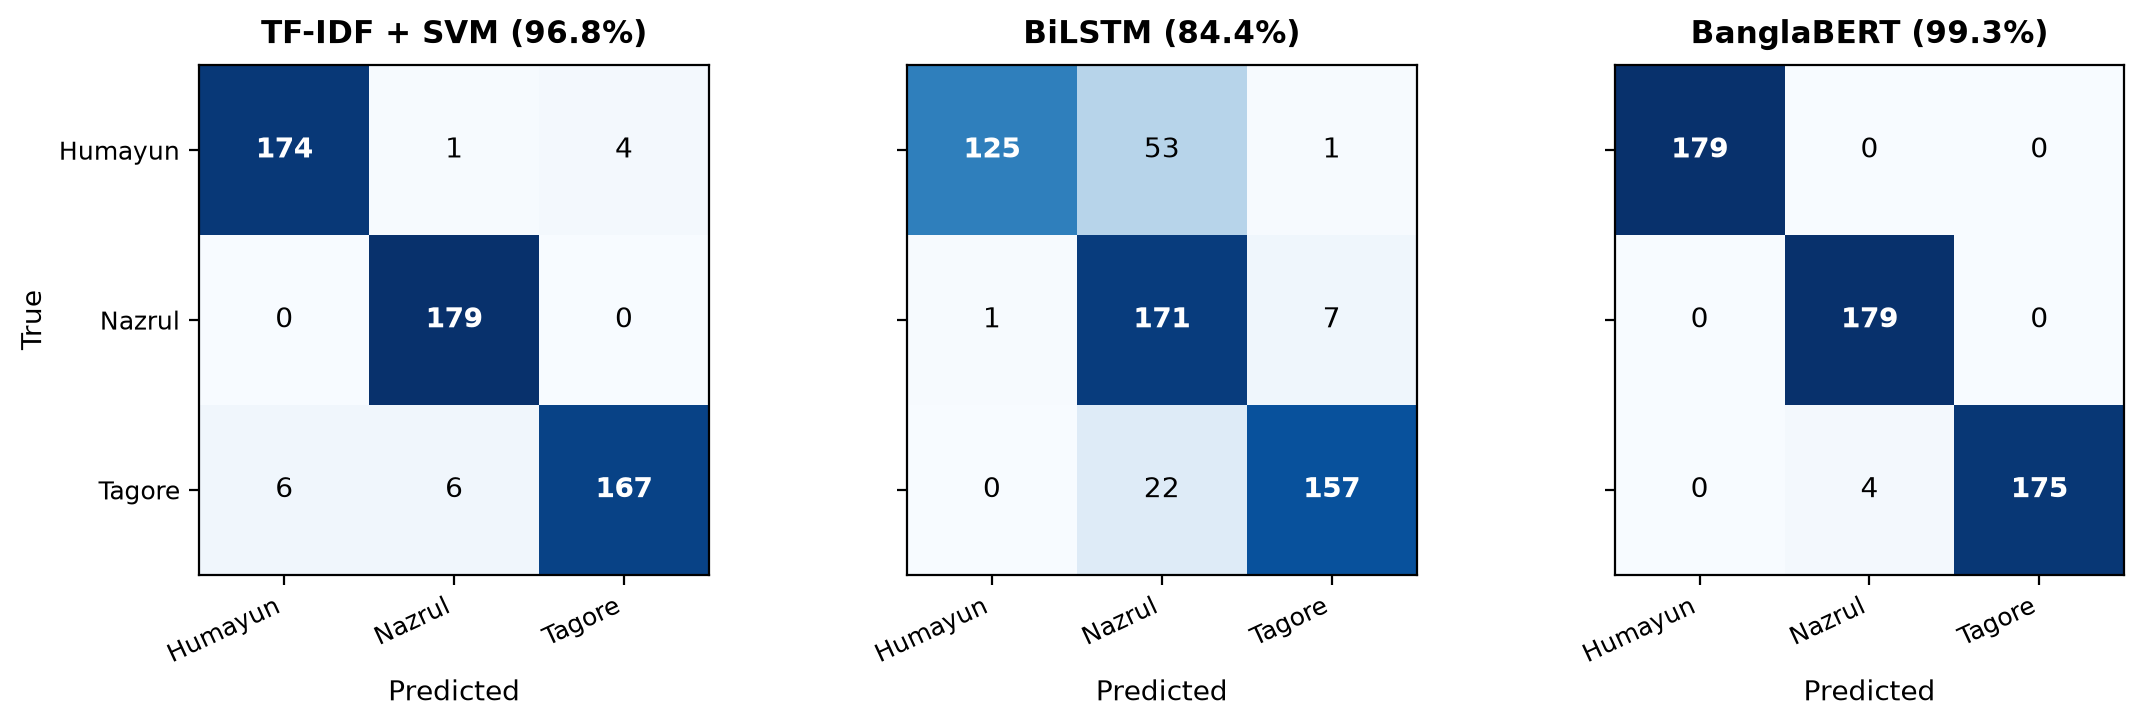
\includegraphics[width=0.88\linewidth]{figures/confusion_models.png}
\caption{How the models got confused on the unseen books: TF--IDF + SVM (left), BiLSTM (centre), and BanglaBERT (right).}
\label{fig:confusion_models}
\end{figure}

Figure \ref{fig:confusion_models} shows where the models made mistakes on our 537 unseen test passages:
\begin{itemize}
  \item \textbf{TF--IDF + SVM (96.8\%):} It perfectly guessed Nazrul and almost perfectly guessed Humayun. It got slightly confused on Tagore, guessing Humayun or Nazrul a total of 12 times.
  \item \textbf{BiLSTM (82.9\%):} It got very confused, incorrectly guessing that Nazrul wrote 53 of Humayun's passages and 22 of Tagore's passages. Without outside knowledge, this model got tricked by random word patterns.
  \item \textbf{BanglaBERT (98.5\%):} It was nearly perfect. It scored 100\% on Humayun and Nazrul, and only mislabeled 4 of Tagore's passages as Nazrul.
\end{itemize}

Even though BanglaBERT is the most accurate, we kept the simpler models around because they can explain \emph{why} they made their choice.

Naive Bayes and SVM models do math that we can easily trace. We can see exactly which words or features gave points to each author. We can show a user the exact words in their text that made the model pick Humayun over Tagore.

BanglaBERT cannot explain its choices this clearly. It is highly accurate, but it acts like a black box. Our report highlights this trade-off between being accurate and being understandable.

The features that separate these three authors are things a Bengali reader would notice immediately. For example, \longestSentAuthor{} writes long sentences averaging \longestSentLen{} words, while \shortestSentAuthor{} writes short sentences averaging \shortestSentLen{} words. Also, older authors use more \bn{সাধু} (literary) words, while modern authors write in a more \bn{চলিত} (colloquial) style and use more dialogue.

\section{The web app}

We built a web interface to let anyone try out our system. The app shows three things:

\begin{itemize}
  \item the \textbf{dataset}, listing our books and letting you read sample paragraphs;
  \item the \textbf{steps} our system takes, showing how text is processed;
  \item the \textbf{results}, letting you paste in text and see the guesses from TF-IDF, BiLSTM, and BanglaBERT side-by-side.
\end{itemize}

The main point of the app is to show all three models at once. If they all agree, you can be very confident. If they disagree (which often happens on short texts), the app shows you the disagreement instead of hiding it behind one single guess.

The app pulls sample text directly from our unseen books. This ensures that the models are always guessing on text they have never seen before, making it a fair test.

\section{Limitations to keep in mind}
\label{sec:limitations}

\paragraph{It only knows three authors.} If you give the system a text written by a fourth author, it will still confidently guess one of our three authors. It doesn't have an "I don't know" option.

\paragraph{Time period affects the score.} Our authors lived between 1861 and 2012. They use different spelling rules and levels of formality. Part of our high score comes from the model guessing the \emph{time period}, not just the personal style. If we tested three authors from the same exact time period, our scores would definitely be lower.

\paragraph{Vocabulary is doing heavy lifting.} Just looking at the words (TF-IDF) gets us a \tfidfBaselineAcc{} accuracy. We openly admit that vocabulary alone solves most of the problem here.

\paragraph{Small dataset.} We only used six training books, and our smallest author had very little text. Our poor BiLSTM results are mostly because we didn't have enough data, not because the model architecture is bad.

\paragraph{Validation is easier than the real test.} Our validation set is made of chapters from our training books. It only checks if the model can generalize to new chapters, not to completely new books. It scores higher than our real test, so we only use it to guide our training, never as a final result.

\section{Conclusion}

We tested our models on \nTest{} passages from \nUnseenBooks{} books they had never seen before. Our models scored anywhere from \bilstmAcc{} to \bertFTAcc{}, all beating the \chanceAcc{} chance of random guessing. We found three big takeaways:

First, \textbf{complexity does not guarantee accuracy}. Our complicated BiLSTM did worse than a simple word counter because it didn't have enough data to learn from scratch. On a small dataset, giving a model pre-trained knowledge (like BanglaBERT) is much more important than the model's structure.

Second, \textbf{how you test is more important than what you test}. The same exact model scored \randomSplitAcc{} when we tested it sloppily, and \workSplitAcc{} when we tested it strictly on unseen books. A bad test setup will give you a fake perfect score and trick you into thinking a memorizing model is actually smart.

Third, \textbf{always check your data}. We found that \nOverlapHits{} stories were reprinted in both our training and test books. If we hadn't built a tool to scan the actual text and remove them, all our results would have been ruined. You cannot just trust book titles or metadata.


\end{document}
